\documentclass[letterpaper,11pt,twoside]{article}
\usepackage[utf8]{inputenc}
\usepackage{amsmath,amsfonts,amssymb,amsthm,latexsym}
\usepackage[spanish,es-noshorthands]{babel}
\usepackage[T1]{fontenc}
\usepackage{lmodern}
\usepackage{graphicx,hyperref}
\usepackage{tikz,pgf}
\usepackage{marvosym}
\usepackage{multicol}
\usepackage{fancyhdr}
\usepackage[final]{pdfpages}
\usepackage[height=9.5in,width=7in]{geometry}
\usepackage{fancyhdr}
\pagestyle{fancy}
\fancyhead[LE]{\Email matematicas.german@gmail.com}
\fancyhead[RE]{\url{https://www.autistici.org/mathgerman}}
\fancyhead[RO]{\url{https://www.autistici.org/mathgerman}}
\fancyhead[LO]{\Email matematicas.german@gmail.com}

\author{Germ\'an Avenda\~no Ram\'irez~\thanks{Lic. Mat. U.D., M.Sc. U.N.}}
\title{\begin{minipage}{.2\textwidth}

\includegraphics[height=1.75cm]{Images/logo-colegio.png}\end{minipage}
\begin{minipage}{.55\textwidth}
\begin{center}
Recomendaciones iii período\\
Matemáticas $11^{\circ}$
\end{center}
\end{minipage}\hfill
\begin{minipage}{.2\textwidth}

\includegraphics[height=1.75cm]{Images/logo-sed.png} 
\end{minipage}}
\date{}
\thispagestyle{plain}
\begin{document}
\maketitle
Nombre: \hrulefill Curso: \underline{\hspace*{44pt}} Fecha: \underline{\hspace*{2.5cm}}
\begin{multicols}{2}
\section*{Cálculo}
\begin{enumerate}
\item Explique con sus propias palabras, que significa la ecuación 
\[\displaystyle{\lim_{x\rightarrow 2}f(x)=5}\]
¿Es posible que esto pueda ser verdadero aunque $f(2)=3$? Explique.
\item Explique que significa decir que:
\[\displaystyle{\lim_{x\rightarrow 1^{-}}f(x)=3}\quad \text{and} \quad \displaystyle{\lim_{x \rightarrow 1^{+}}f(x)=7}\]
En esta situación, ¿es posible que $\displaystyle{\lim_{x\rightarrow 1}f(x)}$ exista? Explique

Para los ejercicios \ref{q01}--\ref{q02}, use una tabla de valores para estimar el valor del límite. Luego use Geogebra para confirmar su resultado gráficamente.
\item \label{q01} $\displaystyle{\lim_{x\rightarrow 2}\dfrac{x-2}{x^{2}-3x+2}}$
\item $\displaystyle{\lim_{x\rightarrow 0}\dfrac{2^{x}-1}{x}}$
\item \label{q02} $\displaystyle{\lim_{x\rightarrow 1^{+}}\ln\sqrt{x-1} }$
\item La gráfica de $f$ se muestra en la figura. Encuentre cada límite o explique por qué no existe.
\begin{center}
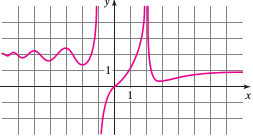
\includegraphics[scale=.75]{Images/Screenshot01.png} 
\end{center}
\begin{enumerate}
\begin{multicols}{2}
\item $\displaystyle{\lim_{x\rightarrow 2^{+}}f(x)}$
\item $\displaystyle{\lim_{x\rightarrow 3^{+}}f(x)}$
\item $\displaystyle{\lim_{x\rightarrow 3^{-}}f(x)}$
\item $\displaystyle{\lim_{x\rightarrow -3}f(x)}$
\item $\displaystyle{\lim_{x\rightarrow 4}f(x)}$
\item $\displaystyle{\lim_{x\rightarrow 0}f(x)}$
\item $\displaystyle{\lim_{x\rightarrow \infty}f(x)}$
\item $\displaystyle{\lim_{x\rightarrow -\infty}f(x)}$
\end{multicols}
\end{enumerate}
\item Sea \[f(x)= \left\{ \begin{array}{lcl}
2 & \mbox{ si } & x<-1 \\
x^{2} & \mbox{ si } & -1\leq x\leq 2\\
x+2 & \mbox{ si } & x>2
\end{array}
\right.\]
Encuentre cada límite o explique por qué no existe
\begin{enumerate}
\begin{multicols}{2}
\item $\displaystyle{\lim_{x\rightarrow -1^{-1}}f(x)}$
\item $\displaystyle{\lim_{x\rightarrow -1^{+}}f(x)}$
\item $\displaystyle{\lim_{x\rightarrow -1}f(x)}$
\item $\displaystyle{\lim_{x\rightarrow 2^{-}}f(x)}$
\item $\displaystyle{\lim_{x\rightarrow 2^{+}}f(x)}$
\item $\displaystyle{\lim_{x\rightarrow 2}f(x)}$
\item $\displaystyle{\lim_{x\rightarrow 0}f(x)}$
\item $\displaystyle{\lim_{x\rightarrow 3}(f(x))^{2}}$
\end{multicols}
\end{enumerate}
\ref{q03}--\ref{q04}, use las propiedades de los límites para evaluar el límite si existe
\begin{multicols}{2}
\item \label{q03} $\displaystyle{\lim_{x\rightarrow 2}\dfrac{x+1}{x-3}}$
\item $\displaystyle{\lim_{t\rightarrow 1}(t^{3}-3t+6)}$
\item $\displaystyle{\lim_{x\rightarrow 3}\dfrac{x^{2}+x-12}{x-3}}$
\item $\displaystyle{\lim_{x\rightarrow -2}\dfrac{x^{2}-4}{x^{2}+x-2}}$
\item $ \displaystyle{\lim_{u\rightarrow 0}\dfrac{(u+1)^{2}-1}{u}}$
\item $\displaystyle{\lim_{z\rightarrow 9}\dfrac{\sqrt{z}-3}{z-9}}$
\item $\displaystyle{\lim_{x\rightarrow 3^{-}}\dfrac{x-3}{|x-3|}}$
\item $\displaystyle{\lim_{x\rightarrow 0}\left(\dfrac{1}{x}+\dfrac{2}{x^{2}-2x}\right)}$
\item $\displaystyle{\lim_{x\rightarrow \infty}\dfrac{2x}{x-4}}$
\item \label{q04} $\displaystyle{\lim_{x\rightarrow \infty}\dfrac{x^{2}+1}{x^{4}-3x+6}}$
\end{multicols}
\end{enumerate}
\section*{Probabilidad}
Resolver los ejercicios 1.81 a 1.94
\end{multicols}
\includepdfmerge{11_prob_recom_iii.pdf,1-2} 
\end{document}
